\section{Distribution of IVOA Virtual Observatories Worlwide and its Projects}
\subsection{The IVOA}
From June 2002, projects of virtual observatories have come to integrate the
International Virtual Observatory Alliance (IVOA) under the \textbf{Guidelines
for Participation\footnote{The guidelines are available in a paper in PDF and
DOC format from
\url{http://www.ivoa.net/documents/latest/IVOAParticipation.html}}}. These were
founded through national and international governmental and private programs in
collaboration with various centers of scientific studies, universities and
others. Who integrate this project, the Virtual Observatory (VO), share
knowledge between them and the community in a standardized manner. They
themselves are who develop these standards for data exchange and
interoperability. The table \ref{table:partners} shows the partners of IVOA to
November 2013.\\

\begin{table}%[h!t]
\centering
\begin{tabular}{|p{7cm}|p{7cm}|}
	\hline
	\textbf{Project} & \textbf{URL} \\
	\hline
	Argentina Virtual Observatory & \url{http://nova.conicet.gov.ar/} \\
	\hline
	Armenian Virtual Observatory & \url{http://www.aras.am/Arvo/arvo.htm} \\
	\hline
	AstroGrid & \url{http://www.astrogrid.org/} \\
	\hline
	Australian Virtual Observatory & \url{http://aus-vo.org.au/} \\
	\hline
	Brazilian Virtual Observatory & \url{http://www.lna.br/bravo/} \\
	\hline
    Canadian Virtual Observatory &
    \url{http://www.cadc-ccda.hia-iha.nrc-cnrc.gc.ca/cvo/} \\
	\hline
    Chilean Virtual Observatory & \url{http://www.chivo.cl/} \\
	\hline
    Chinese Virtual Observatory &
    \url{http://www.china-vo.org/} \\
	\hline
    European Space Agency &
    \url{http://www.sciops.esa.int/index.php?project=ESAVO} \\
	\hline
	European Virtual Observatory & \url{http://www.euro-vo.org/} \\
	\hline
	German Astrophysical Virtual Observatory & \url{http://www.g-vo.org/} \\
	\hline
	Hungarian Virtual Observatory & \url{http://hvo.elte.hu/en/} \\
	\hline
	Italian Virtual Observatory & \url{http://vobs.astro.it/} \\
	\hline
	Japanese Virtual Observatory & \url{http://jvo.nao.ac.jp/}\\
	\hline
	Observatorie Virtuel France & \url{http://www.france-vo.org/} \\
	\hline
	Russian Virtual Observatory & \url{http://www.inasan.rssi.ru/eng/rvo/} \\
	\hline
	Spanish Virtual Observatory & \url{http://svo.cab.inta-csic.es/} \\
	\hline
	South African Astroinformatics Alliance & \url{http://www.sa3.ac.za/} \\
	\hline
	Ukranian Virtual Observatory & \url{http://www.ukr-vo.org/} \\
	\hline
	Virtual Astronomical Observatory & \url{http://www.usvao.org/} \\
	\hline
	Virtual Observatory India & \url{http://vo.iucaa.ernet.in/~voi/} \\
	\hline
\end{tabular}
\caption{IVOA's partners.}
\label{table:partners}
\end{table}

Almost half of IVOA virtual observatories are supported in Europe\footnote{The
Observatoire Virtuel France is ommited in \textbf{Europe} subsection of
\textbf{List of Virtual Observatories} section by lack of the information.} 9 of
the total; 1 belong to Africa, 1 to Australia, 2 to North America, 3 to South
America and 5 to Asia\footnote{As the mayor part of Rusia's territory is in
Asia, it will be considered like a virtual observatory of Asian continent.}. The
figure 1 shows the distribution of the IVOA's membership per continent.\\

\begin{figure}%[h]
\begin{center}
	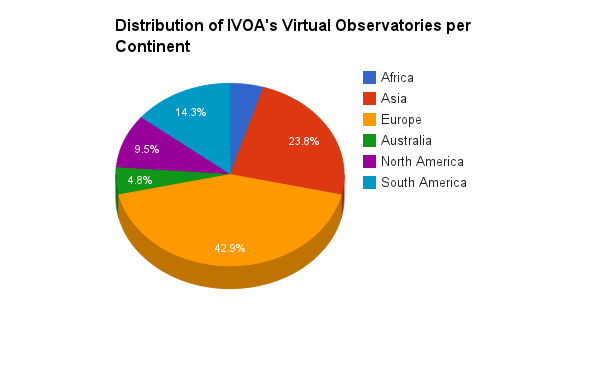
\includegraphics[scale=0.6]{img/vo_distribution.png}
	\caption{International Virtual Observatory Alliance distribution per
             continent.}
\end{center}
\end{figure}

% If Chile became part of International Virtual Observatory Alliance, the
% distribution of IVOA's members per continent will be as shown in the figure
% 2. \\

%\begin{comment}
\begin{figure}%[h]
\begin{center}
	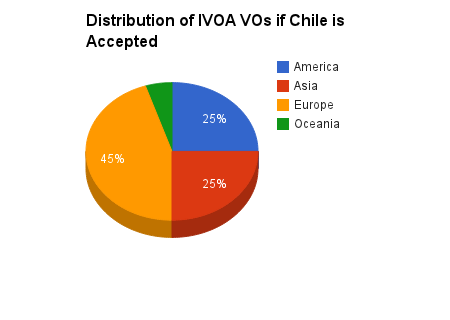
\includegraphics[width=110mm]{img/if_chile.png}
	\caption{International Virtual Observatory Alliance distribution per
             continent if Chile is accepted.}
\end{center}
\end{figure}
%\end{comment}

Without considering the status of the internal projects of the virtual
observatories, the membership of Chile would contribute to the cooperation,
development and interoperability from America in the same percent that Asia.
Furthermore, this fact would be very significant, because a large numbers of
astronomical centers like observatories are placed in this country.  For now, is
intended to work with a certain quantity of data of ALMA.\\
